\documentclass[12pt, openany]{report}
\usepackage[T1]{fontenc}
\usepackage[english, french]{babel}
\usepackage{csquotes}
\usepackage[margin=2.5cm]{geometry}
\usepackage{setspace}
\usepackage{microtype}
\usepackage{amsmath, amssymb, amsthm}
\usepackage{graphicx}
\usepackage{booktabs}
\usepackage[style=authoryear]{biblatex}
\addbibresource{references.bib}
\usepackage[colorlinks=true, allcolors=blue]{hyperref}

\onehalfspacing

\begin{document}

\pagenumbering{alph}
\begin{titlepage}
  \centering
  {\large\scshape Établissement \par}
  {\large Département \par}
  \vspace{3cm}
  {\huge\bfseries {{TITLE}} \par}
  \vspace{2cm}
  {\Large {{AUTHOR}} \par}
  \vspace{2cm}
  Mémoire présenté en vue de l'obtention du diplôme de \par
  maîtrise ès sciences appliquées \par
  \vspace{1cm}
  Sous la direction de Nom du directeur ou de la directrice \par
  \vfill
  {\large \today \par}
\end{titlepage}

\pagenumbering{roman}
\chapter*{Remerciements}
\addcontentsline{toc}{chapter}{Remerciements}

Les remerciements nomment les personnes et les organismes qui ont soutenu ce
travail.

\chapter*{Résumé}
\addcontentsline{toc}{chapter}{Résumé}

Le résumé présente en une page la problématique, la méthode, les résultats
et les conclusions du mémoire.

\begin{otherlanguage}{english}
\chapter*{Abstract}
\addcontentsline{toc}{chapter}{Abstract}

The abstract gives the same summary in English.
\end{otherlanguage}

\tableofcontents
\listoffigures
\listoftables

\cleardoublepage
\pagenumbering{arabic}
% Chaque chapitre est dans son propre fichier du dossier chapitres.
\chapter{Introduction}
\label{chap:introduction}

L'introduction présente le contexte, la problématique et les objectifs du
mémoire, puis en annonce le plan: le chapitre~\ref{chap:revue} passe en revue
les travaux existants, le chapitre~\ref{chap:methode} décrit la méthode et
le chapitre~\ref{chap:conclusion} conclut.

Chaque chapitre est un fichier du dossier \texttt{chapitres}, inclus dans
\texttt{main.tex} par une commande \verb|\include|.

\chapter{Revue de la littérature}
\label{chap:revue}

Ce chapitre situe le mémoire parmi les travaux existants. Les références
se trouvent dans le fichier \texttt{references.bib}. Ainsi,
\textcite{knuth1984} décrit \TeX{} et \textcite{lamport1994} présente
\LaTeX{}. On peut aussi citer entre parenthèses \parencite{mittelbach2023}.

\chapter{Méthode et résultats}
\label{chap:methode}

\section{Méthode}

La méthode s'appuie sur le modèle
\begin{equation}
  \label{eq:modele}
  \frac{\mathrm{d}x}{\mathrm{d}t} = -\lambda x, \qquad x(0) = x_0,
\end{equation}
dont la solution est $x(t) = x_0 e^{-\lambda t}$.

\section{Résultats}

La figure~\ref{fig:resultats} et le tableau~\ref{tab:resultats} présentent
les résultats obtenus avec le modèle~\eqref{eq:modele}.

\begin{figure}[htbp]
  \centering
  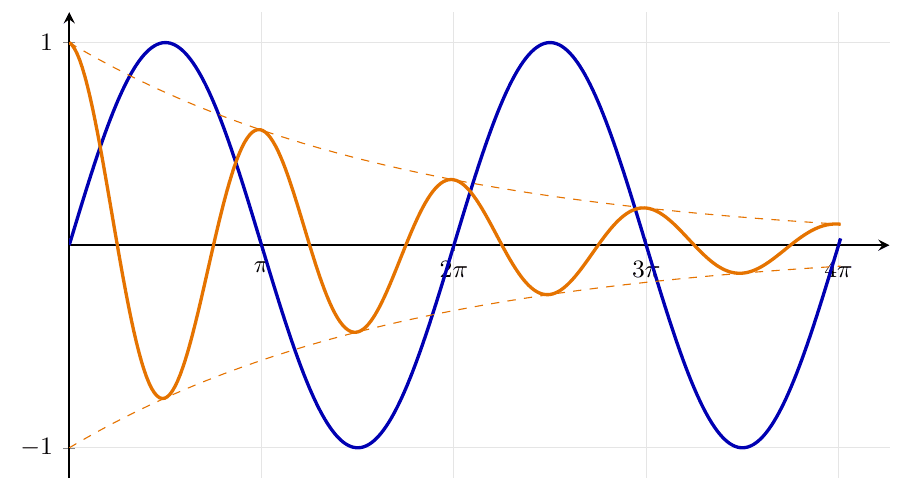
\includegraphics[width=0.75\linewidth]{images/courbes.png}
  \caption{Une image du projet: remplacez-la par vos résultats.}
  \label{fig:resultats}
\end{figure}

\begin{table}[htbp]
  \centering
  \caption{Valeurs estimées du paramètre $\lambda$.}
  \label{tab:resultats}
  \begin{tabular}{lrr}
    \toprule
    Essai & $\lambda$ & Erreur relative (\%) \\
    \midrule
    1 & 0,182 & 1,1 \\
    2 & 0,179 & 0,6 \\
    3 & 0,185 & 2,8 \\
    \bottomrule
  \end{tabular}
\end{table}

\chapter{Conclusion}
\label{chap:conclusion}

La conclusion résume les contributions du mémoire, en discute les limites et
propose des pistes de recherche.


\printbibliography[heading=bibintoc]

\appendix
\chapter{Données complémentaires}
\label{chap:annexe}

Les annexes rassemblent les démonstrations longues, les données et le code.


\end{document}
